\documentclass{article}

\usepackage{graphicx}
\usepackage{tikz}
\usepackage{tikzsymbols}
\usetikzlibrary{calc,patterns,shapes.geometric}
\pagestyle{empty}
\usepackage[margin=0pt]{geometry}
\geometry{papersize={14in,12in}}

\def\centerarc[#1](#2)(#3:#4:#5){\draw[#1] ($(#2)+({#5*cos(#3)},{#5*sin(#3)})$) arc (#3:#4:#5);}

\begin{document}
	\begin{figure}
		\centering
		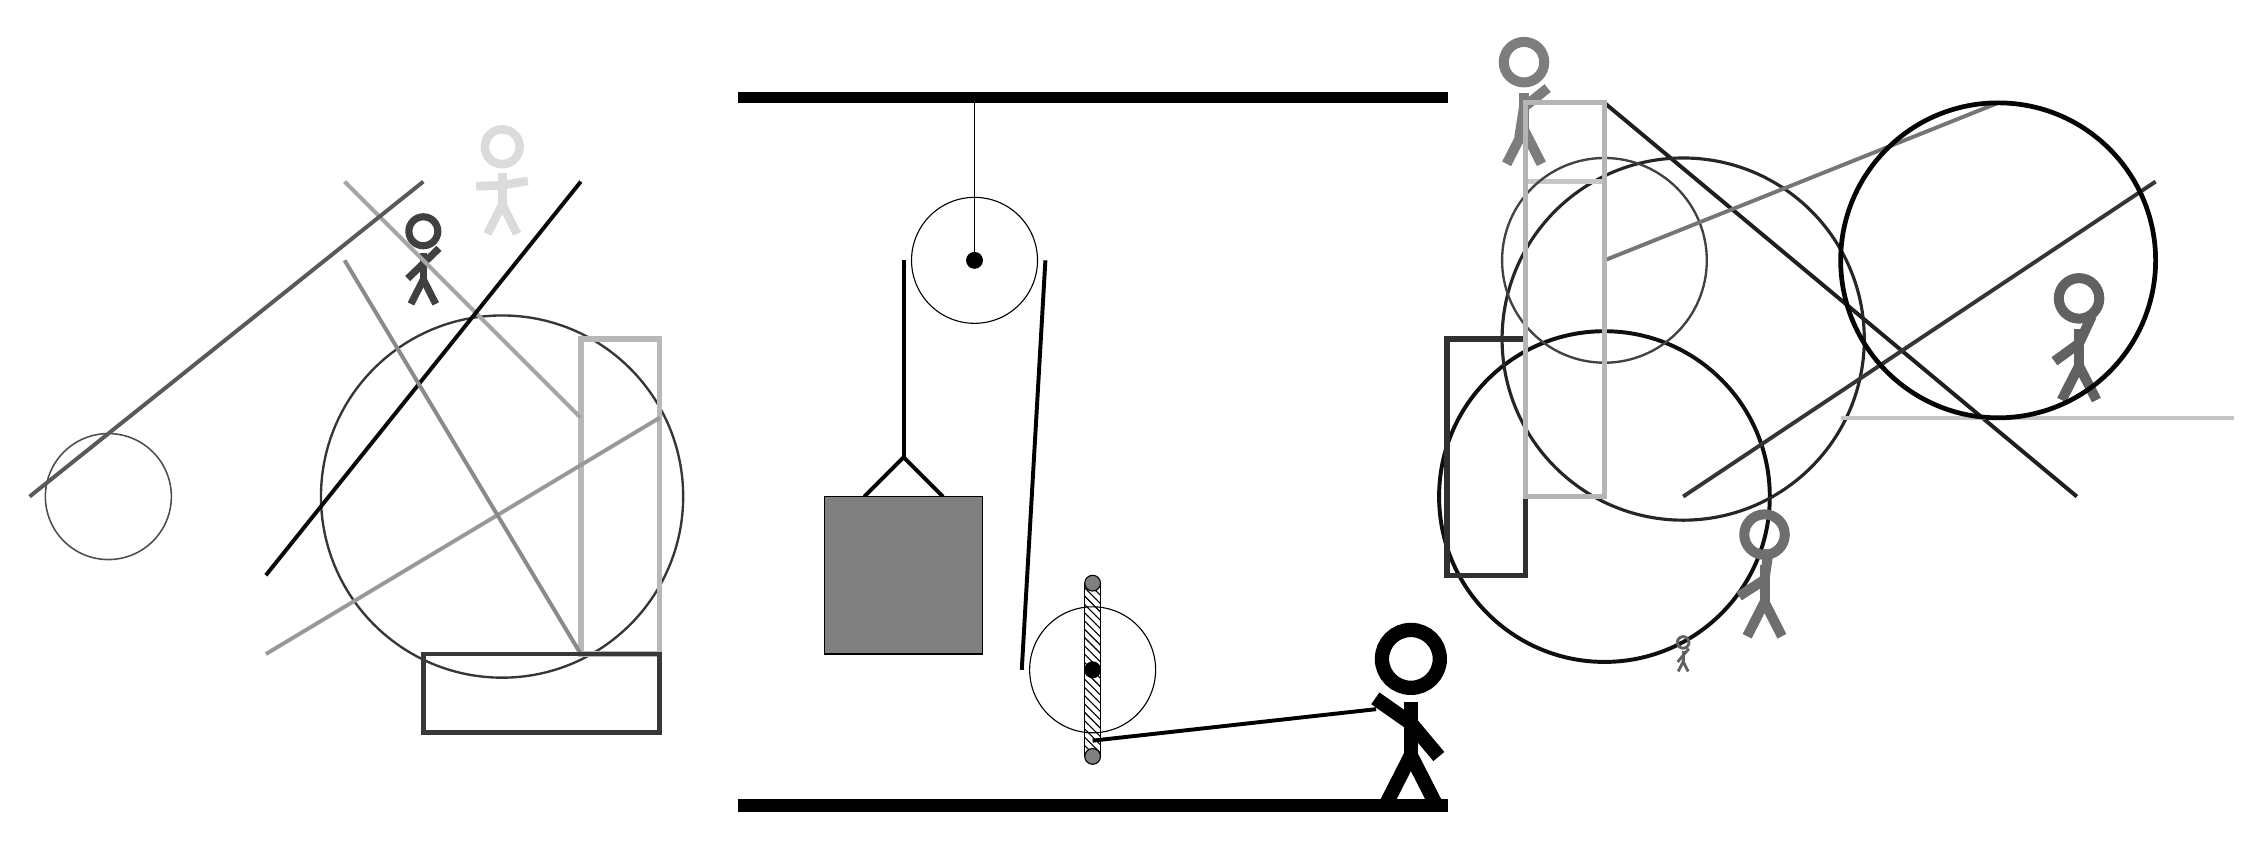
\begin{tikzpicture}
			%%%%% START %%%%%
			
			\draw[fill=black] (-2, 9) rectangle (7, 9.125);
			
			\draw (1, 7) circle (0.8);
			\draw[fill=black] (1, 7) circle (0.1);
			\draw (1, 9) -- (1, 7);
			
			\draw[fill=white](2.5, 1.8) circle (0.8);
			\draw[fill=black] (2.5, 1.8) circle (0.1);
			\draw[pattern=north west lines, pattern color=black] (2.4, 2.9) rectangle (2.6, 0.7);
			\draw[fill=black!50] (2.5, 2.9) circle (0.1);
			\draw[fill=black!50] (2.5, 0.7) circle (0.1);
			
			\draw[line width=0.5mm] (-0.4, 4.0) -- (0.1, 4.5) -- (0.6, 4.0);
			\draw[fill=black!50] (-0.9, 4.0) rectangle (1.1, 2.0);
			
			\draw[line width=0.5mm, color=black!88](9, 9) -- (15, 4);
			
			\draw [line width=0.3mm, color=black!79](-5, 4) circle (2.3);
			\draw [line width=0.5mm, color=black!94](9, 4) circle (2.1);
			\draw[line width=0.6mm, color=black!54] (-3, 6) rectangle (-3, 3);
			\node[line width=0.3mm, color=black!57] at (11, 3) {\Strichmaxerl[7][33][82]};
			\node[line width=0.6mm, color=black!62] at (10, 2) {\Strichmaxerl[2][50][49]};
			
			\draw[line width=0.7mm, color=black!28] (-3, 2) rectangle (-4, 6);
			\draw [line width=0.4mm, color=black!85](10, 6) circle (2.3);
			\node[line width=0.6mm, color=black!75] at (-6, 7) {\Strichmaxerl[5][44][44]};
			
			\draw[line width=0.5mm, color=black!23](12, 5) -- (17, 5);
			\draw[line width=0.5mm, color=black!35](-4, 5) -- (-7, 8);
			\node[line width=0.3mm, color=black!51] at (8, 9) {\Strichmaxerl[7][81][39]};
			\draw[line width=0.5mm, color=black!79](10, 4) -- (16, 8);
			\draw [line width=0.2mm, color=black!69](-10, 4) circle (0.8);
			\draw[line width=0.6mm, color=black!22] (8, 8) rectangle (9, 4);
			\draw[line width=0.5mm, color=black!40](-3, 5) -- (-8, 2);
			
			\draw[line width=0.5mm, color=black!96](-4, 8) -- (-8, 3);
			
			\draw[line width=0.5mm, color=black!46](-4, 2) -- (-7, 7);
			\draw [line width=0.3mm, color=black!74](9, 7) circle (1.3);
			
			\node[line width=0.2mm, color=black!62] at (15, 6) {\Strichmaxerl[7][36][65]};
			\draw[line width=0.5mm, color=black!54](9, 7) -- (14, 9);
			\draw[line width=0.5mm, color=black!65](-6, 8) -- (-11, 4);
			\draw[line width=0.7mm, color=black!81] (7, 3) rectangle (8, 6);
			\node[line width=0.6mm, color=black!14] at (-5, 8) {\Strichmaxerl[6][2][10]};
			\draw [line width=0.6mm, color=black!98](14, 7) circle (2.0);
			
			\draw[line width=0.6mm, color=black!78] (-3, 1) rectangle (-6, 2);
			\draw[line width=0.5mm, color=black!81](-3, 6) -- (-3, 6);
			\draw [line width=0.4mm, color=black!54](-4, 5) circle (0.0);
			\draw[line width=0.6mm, color=black!29] (8, 4) rectangle (9, 9);
			
			
			\draw[line width=0.5mm] (0.1, 7) -- (0.1, 4.5);
			\centerarc[line width=0.5mm](1, 7)(0:180:0.9);
			\draw[line width=0.5mm](1.9, 7) -- (1.6, 1.8);
			\centerarc[line width=0.5mm](2.5, 1.8)(180:270:0.9);
			\draw[line width=0.5mm](2.5, 0.9) -- (6.1, 1.3);
			
			\node at (6.5, 1.2) {\Strichmaxerl[10][-35][-50]};
			
			\draw[fill=black] (-2, 0) rectangle (7, 0.15);
			
			%%%%% END %%%%%
		\end{tikzpicture}
	\end{figure}	
\end{document}